\documentclass[10pt,letterpaper]{article}

\usepackage{hyperref, breakurl}
\usepackage{cogsci}
\usepackage{pslatex}
\usepackage{apacite}
\usepackage{graphicx}
\usepackage{caption}
\usepackage{subcaption}
\usepackage{color}
\usepackage{amsfonts}
\usepackage{amsmath}

\newcommand{\w}[1]{\emph{#1}}
\newcommand{\todo}[1]{{\color{red}#1}}

\title{Extremely costly intensifiers are stronger than quite costly ones}
 
\author{{\large \bf Erin Bennett} (erindb@stanford.edu), {\large \bf Noah D.~Goodman} (ngoodman@stanford.edu)\\
  Department of Psychology, Stanford University.}
  %450 Serra Mall , Stanford, CA 94305}
  
\begin{document}

\maketitle

\begin{abstract}

We show how the wide range in strengths of intensifying degree adverbs (e.g.~\w{very} and \w{extremely}) could be explained by pragmatic inference based on differing cost, rather than differing semantics.
This predicts a linear relationship between the meaning of intensifiers and their length and log-frequency.
We test this prediction in two studies, using two different dependent measures, finding that higher cost does predict stronger meanings.
We discuss the implications for
% what does this mean?
adverbial meaning
and the more general question of how extensive non-arbitrary form-meaning association may be in language.

\textbf{Keywords:} 
intensifiers; degree adverbs; scalar adjectives; pragmatics; m-implicature
\end{abstract}

\section{Introduction}

How do different words get their meanings?
For instance, why is an ``extremely good paper'' better than a ``quite good paper''? The traditional answer \cite{saussure} is that different meanings have been arbitrarily and conventionally assigned to the different word forms.
This view has been challenged by a number of examples in which word meaning appears to be non-arbitrarily related to properties of the word.
In some cases, the phonetic form of a word is systematically related to its meaning, for example rounded vowels and voiced consonants tend to refer to round objects \cite{maluma-takete, bouba-kiki, bouba-kiki2, takete-uloomo}. 
In other cases, orthographic form is diagnostic of meaning, for example, speakers of Hebrew who have never seen Chinese characters are nonetheless above chance at matching them to their corresponding Hebrew words \cite{koriat}. 
Similarly, the length of words predicts aspects of their meanings: across languages longer words refer to more complex meanings \cite{lewis}.
In this paper, we explore adjectival intensifiers\footnote{Intensifiers are adverbs that modify scalar adjectives to increase the degree. The word ``intensifier'' is often used to denote the full range of degree adverbs, be they ``amplifiers'', or ``downtoners'' \cite{quirk}. The ``intensifiers'' we are looking at in this paper are, according to this typology, ``amplifiers'' because they increase (rather than decrease) the threshold associated with a gradable predicate. This typology also distinguishes between two different kinds of amplifiers: those that increase an adjective maximally (e.g. \w{completely} and \w{utterly}) and those that merely increase (e.g. \w{greatly} and \w{terribly}). We do not make this distinction. The word ``intensifier'' is sometimes used for a completely different linguistic phenomenon, where a reflexive is used for emphasis, e.g. ``The king himself gave the command,'' which we do not analyze in this paper.}, like \w{extremely} and \w{quite},
as a case study in which to empirically explore the relationship of meaning to factors like word form and distribution of usage.
Intensifiers form a good case study both because they are amenable to simple quantitative measures of meaning (such as the numeric extent to which they shift the interpretation of a scalar adjective) and because theoretical considerations, which we lay out shortly, suggest a relationship between their meaning and their usage cost (e.g., due to frequency and length).

In the next section we start from the model presented by \citeA{lassiter} to explain the meaning of scalar adjectives, like \emph{tall} and \emph{expensive}. This probabilistic Rational Speech Acts \cite{frank,goodman} model describes how a threshold on meaning (e.g.~the minimum price that counts as an \emph{expensive watch}) can be established by pragmatic inference that takes into account statistical background knowledge (such as the distribution of prices for watches). We explore the effect of having multiple versions of the adjective that have the same meaning but different costs, and find a M(arkedness)-implicature \cite{levinson}: more marked (costly to utter) versions will be interpreted as implicating higher values.
This motivates the hypothesis that a major portion of the meaning of intensifiers comes from this process rather than from conventionally associated meanings. Concretely, this predicts that the meanings of intensifiers are influenced by their form (in length) and their distribution (frequency) of usage. The impact of word length is reminiscent of the results of \citeA{lewis}, who studied noun categories. While word frequency is known to have major effects on sentence processing \cite[e.g.]{levy}, the prediction that frequency should affect meaning is more novel.

We confirm, in two experiments, that English intensifiers in adjective phrases are indeed interpreted as much higher degrees (e.g.~in the case of \w{expensive}, higher prices) for both longer and less frequent intensifiers. This holds in quantitative judgments of meaning and in forced comparisons, and across a number of adjectival dimensions. We conclude with a discussion of different interpretations of these phenomena and future directions.

\section{The semantics of intensifying degree adverbs}

Our paper focuses on intensifying degree adverbs applied to scalar adjectives\footnote{Some of these intensifiers can also apply to verbal and nominal predicates, and different restrictions apply for different intensifiers, e.g. \w{I truly like carrots} is an acceptable utterance, whereas \w{I very like carrots} is not. See \citeA{bolinger} for a discussion.}. Scalar adjectives have been described as having a threshold semantics \cite{kennedy}, where, for example, \w{expensive} means ``having a price greater than $\theta$'' and $\theta$ is a semantic variable inferred from context (e.g., \$100). Above the threshold degree $\theta$, the adjective is true of an object, and below, the adjective is false.
\citeA{lassiter} give a formal model of how this threshold might be inferred for a particular context, which we extend to intensifiers.

\subsection{Background}
Previous researchers have proposed that adjective phrases modified by intensifiers have the same semantics as unmodified adjective phrases, except with new, higher thresholds \cite{kennedyMcnally, klein, wheeler}. That is, some threshold, inferred from context, exists above which objects are \w{expensive} and below which they are not, and the intensifier \w{very} determines a new, higher threshold for \w{very expensive}.
They suggest that the intensified thresholds are determined by first collecting the set of objects in the comparison class class for which the bare adjective is true, and then using that as the comparison class to infer a new threshold, i.e. \w{very expensive laptop} means ``expensive for an expensive laptop''. This analysis results in the expected intensification of adjectives (``expensive for an expensive laptop'' has a higher threshold for being true than simply ``expensive for a laptop'') and is appropriately sensitive to different domains (e.g. the absolute difference in price between thresholds for \w{expensive} and \w{very expensive} is much higher in the context of ``That space station is very expensive,'' than in the context of ``That coffee is very expensive.'').
However, this account does not, in and of itself, distinguish between the graded strengths of different intensifiers, for example, \w{very expensive} and \w{phenomenally expensive}.

Intuition suggests that different intensifiers do have different strengths (e.g. \w{outrageously} seems stronger than \w{quite}), and we provide further evidence of this in our experiments, where participants interperet and compare different intensifiers.
It could be that the degree of strength of different intensifiers is conventionally specified by the lexicon. But the semantics must then specify how these entries affect the very flexible threshold of the relevant adjective.
In addition, the multitude of intensifiers \cite{bolinger} and their apparent productivity\footnote{For example, \w{altitidinously expensive} is not in common usage, but one can easily interpret \w{altitidinously} as a novel intensifier.} suggest a more parsimonious solution would be welcome. 
That is, having a lexically determined meaning for each different intensifier might overlook the similarity among words of this class.

We propose instead that each time a scalar adjective is used, in each phrase, it introduces a free threshold variable (that is, a new token threshold is inferred for every time the lexical entry of the adjective is accessed). Further we propose that intensifiers contribute \emph{nothing} to the literal, compositional semantics\footnote{We take this strong view for rhetorical purposes. It is highly likely that some intensifiers have other aspects of meaning.}. This implies that different adjectival phrases (e.g.~``very expensive watch'' and ``extremely expensive watch'') have equivalent meanings, though with thresholds that will be separately assigned based on context. \emph{However}, the intensifiers do affect the production cost of the corresponding sentences, and it is this cost difference that results in meaning differences.

We next outline and extend \citeauthor{lassiter}'s model of scalar adjectives to include several copies of the relevant adjectival phrase, each with its own threshold variable.
We show that simply having different thresholds for different adjective phrases---and being aware of alternative utterances and their relative communicative costs---is sufficient to communicate the wide range of degrees designated by intensifying degree adverbs.

\subsection{Model}

\citeA{lassiter}'s model belongs to the family of Rational Speech Act (RSA) models in which speaker and listener communicate by recursively reasoning about each other's goals and inferences. These models have been shown to account for many phenomena in pragmatics
\cite{frank, goodman}. The adjective model accounts for uncertainty about the adjectival threshold by including a lifted semantic variable, which the pragmatic listener infers at the same time that she infers the speaker's intended meaning. 
We assume every adjective phrase has its own such variable $\theta_i$\footnote{Other versions of this model could easily be imagined in which the threshold for an adjective phrase is determined by the basic threshold for the adjective and some transformation on that threshold (e.g. multiplication, addition, etc.) caused by the intensifier. If the transformation is mostly regular, with a single parameter needing to be inferred for each intensifier, and if the values of these parameters are inferred for each adjective phrase, then such a model would be functionally equivalent to the one we describe here.}, together notated $\vec{\theta}$, but to otherwise mean the same thing, so that, for example, \w{expensive}, \w{very expensive} and \w{phenomenally expensive} all denote: $\lambda x . \text{price}(x) > \theta_i$. %unpack?

Given an utterance $u_i$ (e.g. an \w{expensive laptop} or a \w{very expensive laptop}) and a set of thresholds, a literal listener $L_0$ will use Bayesian inference to update his prior beliefs $P(d)$ about the degree $d$ (e.g. the laptop's price) given that the degree is greater than the threshold for that utterance.

$$P_{L_0}(d|u_i, \theta_i) \propto P(d) \cdot \delta_{d > \theta_i}$$

A speaker with the goal of communicating some actual degree $d$ assigns a utility $\mathbb{U}(u_i|d)$ to each utterance such that he prefers utterances which will inform the literal listener, but avoids utterance cost, $C(u_i)$:

$$\mathbb{U}(u_i | d, \vec{\theta}) =  \ln\left(P_{L_0}(d | u_i, \theta_i) \right) - C(u_i) $$

Given a set of alternative utterances (e.g. the speaker might be choosing between saying \w{very expensive} as opposed to \w{expensive} or \w{extremely expensive}, or saying nothing at all), the speaker $S_1$ will choose utterances according to a softmax decision rule \cite{sutton} with optimality parameter $\lambda$, so that:

$$ P_{S_1}(u_i | d, \vec{\theta}) \propto e^{\lambda \mathbb{U}(u_i | d, \vec{\theta})} $$

A pragmatic listener $L_1$ uses the prior probability, $P(d)$, of different degrees, along with knowledge of the cost of each utterance, in order to guess both the thresholds for each utterance and which degree the speaker intended to communicate\footnote{We assume a uniform prior on thresholds $\theta_i$.}:

$$ P_{L_1}(d, \vec{\theta} | u_i) \propto P(d) \cdot P_{S_1}(u_i | d, \vec{\theta}) $$

As an initial exploration, we simulated such a model with three alternative adjective phrases (i.e.~three intensifiers) with costs of $1$, $5$, and $10$. We also included a null utterance, with trivial meaning (always true) and cost of $0$. The prior distribution of degrees along this adjective's scale (which we will discuss as ``prices'' for concreteness and consistency with our Experiment 1) was a gaussian peaked at $0$.
We used an optimality parameter of $\lambda=5$ in our simulation. 

Though the literal semantics are identical (except that they have different threshold parameters), the different phrases received different interpretations: the more costly intensifiers corresponded to less probable, more extreme prices (Figure ~\ref{model}). This can be seen as an M-implicature: more costly intensifiers are assigned strong, less probable, meanings. 
The model therefore predicts an association between intensifier meaning and utterance cost.

\begin{figure}[ht]
\begin{center}
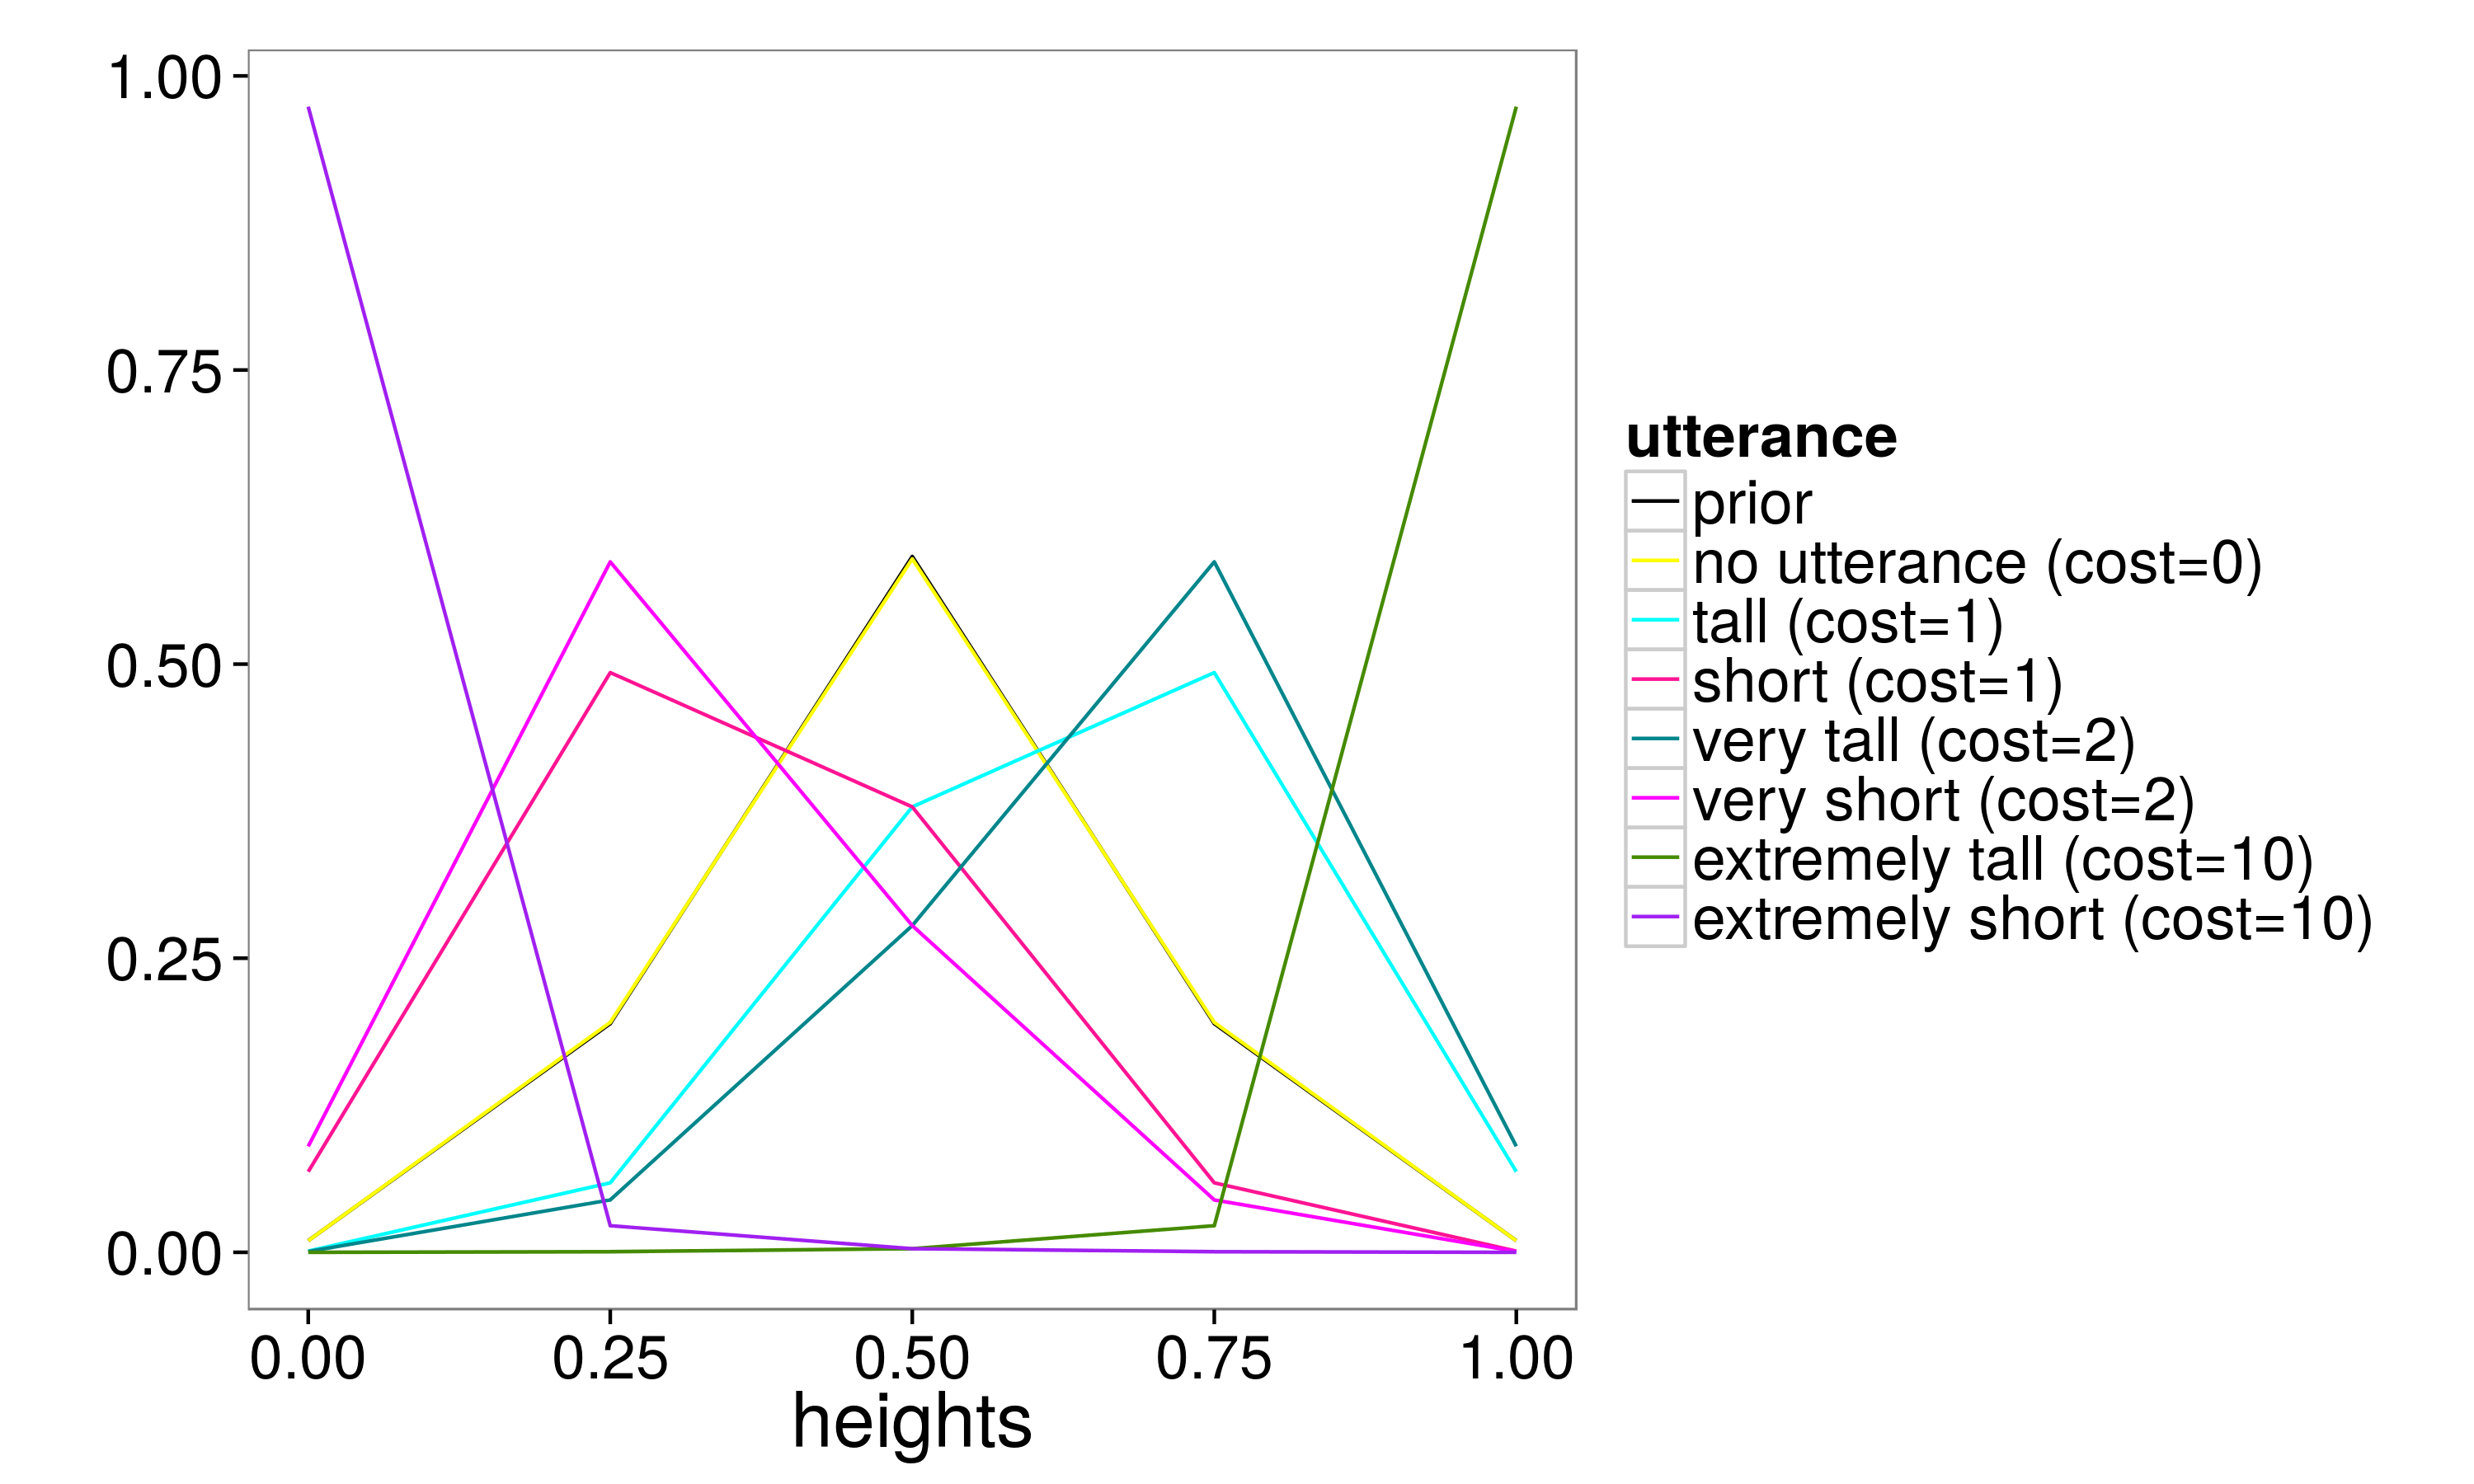
\includegraphics[width=0.48\textwidth]{analysis_files_for_writeup/images/model_results.png}
\end{center}
\caption{Modeling intensifiers as M-implicature: more costly intensifiers correspond to more extreme meanings.} 
\label{model}
\end{figure}

\subsection{Factors affecting utterance cost}

We have identified the intensifier's cost, $C(u_{i})$, as a potentially critical factor of its interpreted meaning. The quantitative form predicted by the model of the relationship between cost and meaning is a approximately linear (Figure \ref{model-heights}).\footnote{This second simulation was identical as the first, except run on a more discretized scale for 6 different utterance costs (or ``intensifiers'').}.

To connect this linear prediction to empirical facts, we still must specify (at least a subset of) the factors we expect to impact cost.
The most natural notion of cost is the effort a speaker incurs to produce an utterance. This could include cognitive effort to access lexical items from memory, articulatory effort to produce 
the sound forms, and other such direct costs.
Speakers might also seek to minimize comprehension cost for their listeners, resulting in other contributions to cost. 
For the purposes of this paper, we restrict to the most
straightforward contributors to production cost and use proxies that are straightforward to quantify: length (longer utterances are more costly)
\footnote{We measure length in number of syllables, although length in characters (which might be a relevant source of utterance cost in a written format, as our experiments were in) has similar predictive power to syllable length in all of our analyses.}
and frequency (rarer intensifiers are harder to access and therefore more costly).
In a number of different tasks, lexical frequency affects difficulty in an approximately logarithmic way. For instance word recognition time \cite{McCusker1977} 
and reading time in context \cite{smithLevy} are both logarithmic in frequency. We thus use the log-frequency (whose negative is also called \emph{surprisal}) as the quantitative contribution to cost.

We thus predict  a linear contribution of longer and higher surprisal intensifiers to the meaning. 
This leaves open the the relative importance of length and surprisal, and potential interactions (as well as other factors that might enter into cost), which can be explored via regression models.


\begin{figure}[ht]
\begin{center}
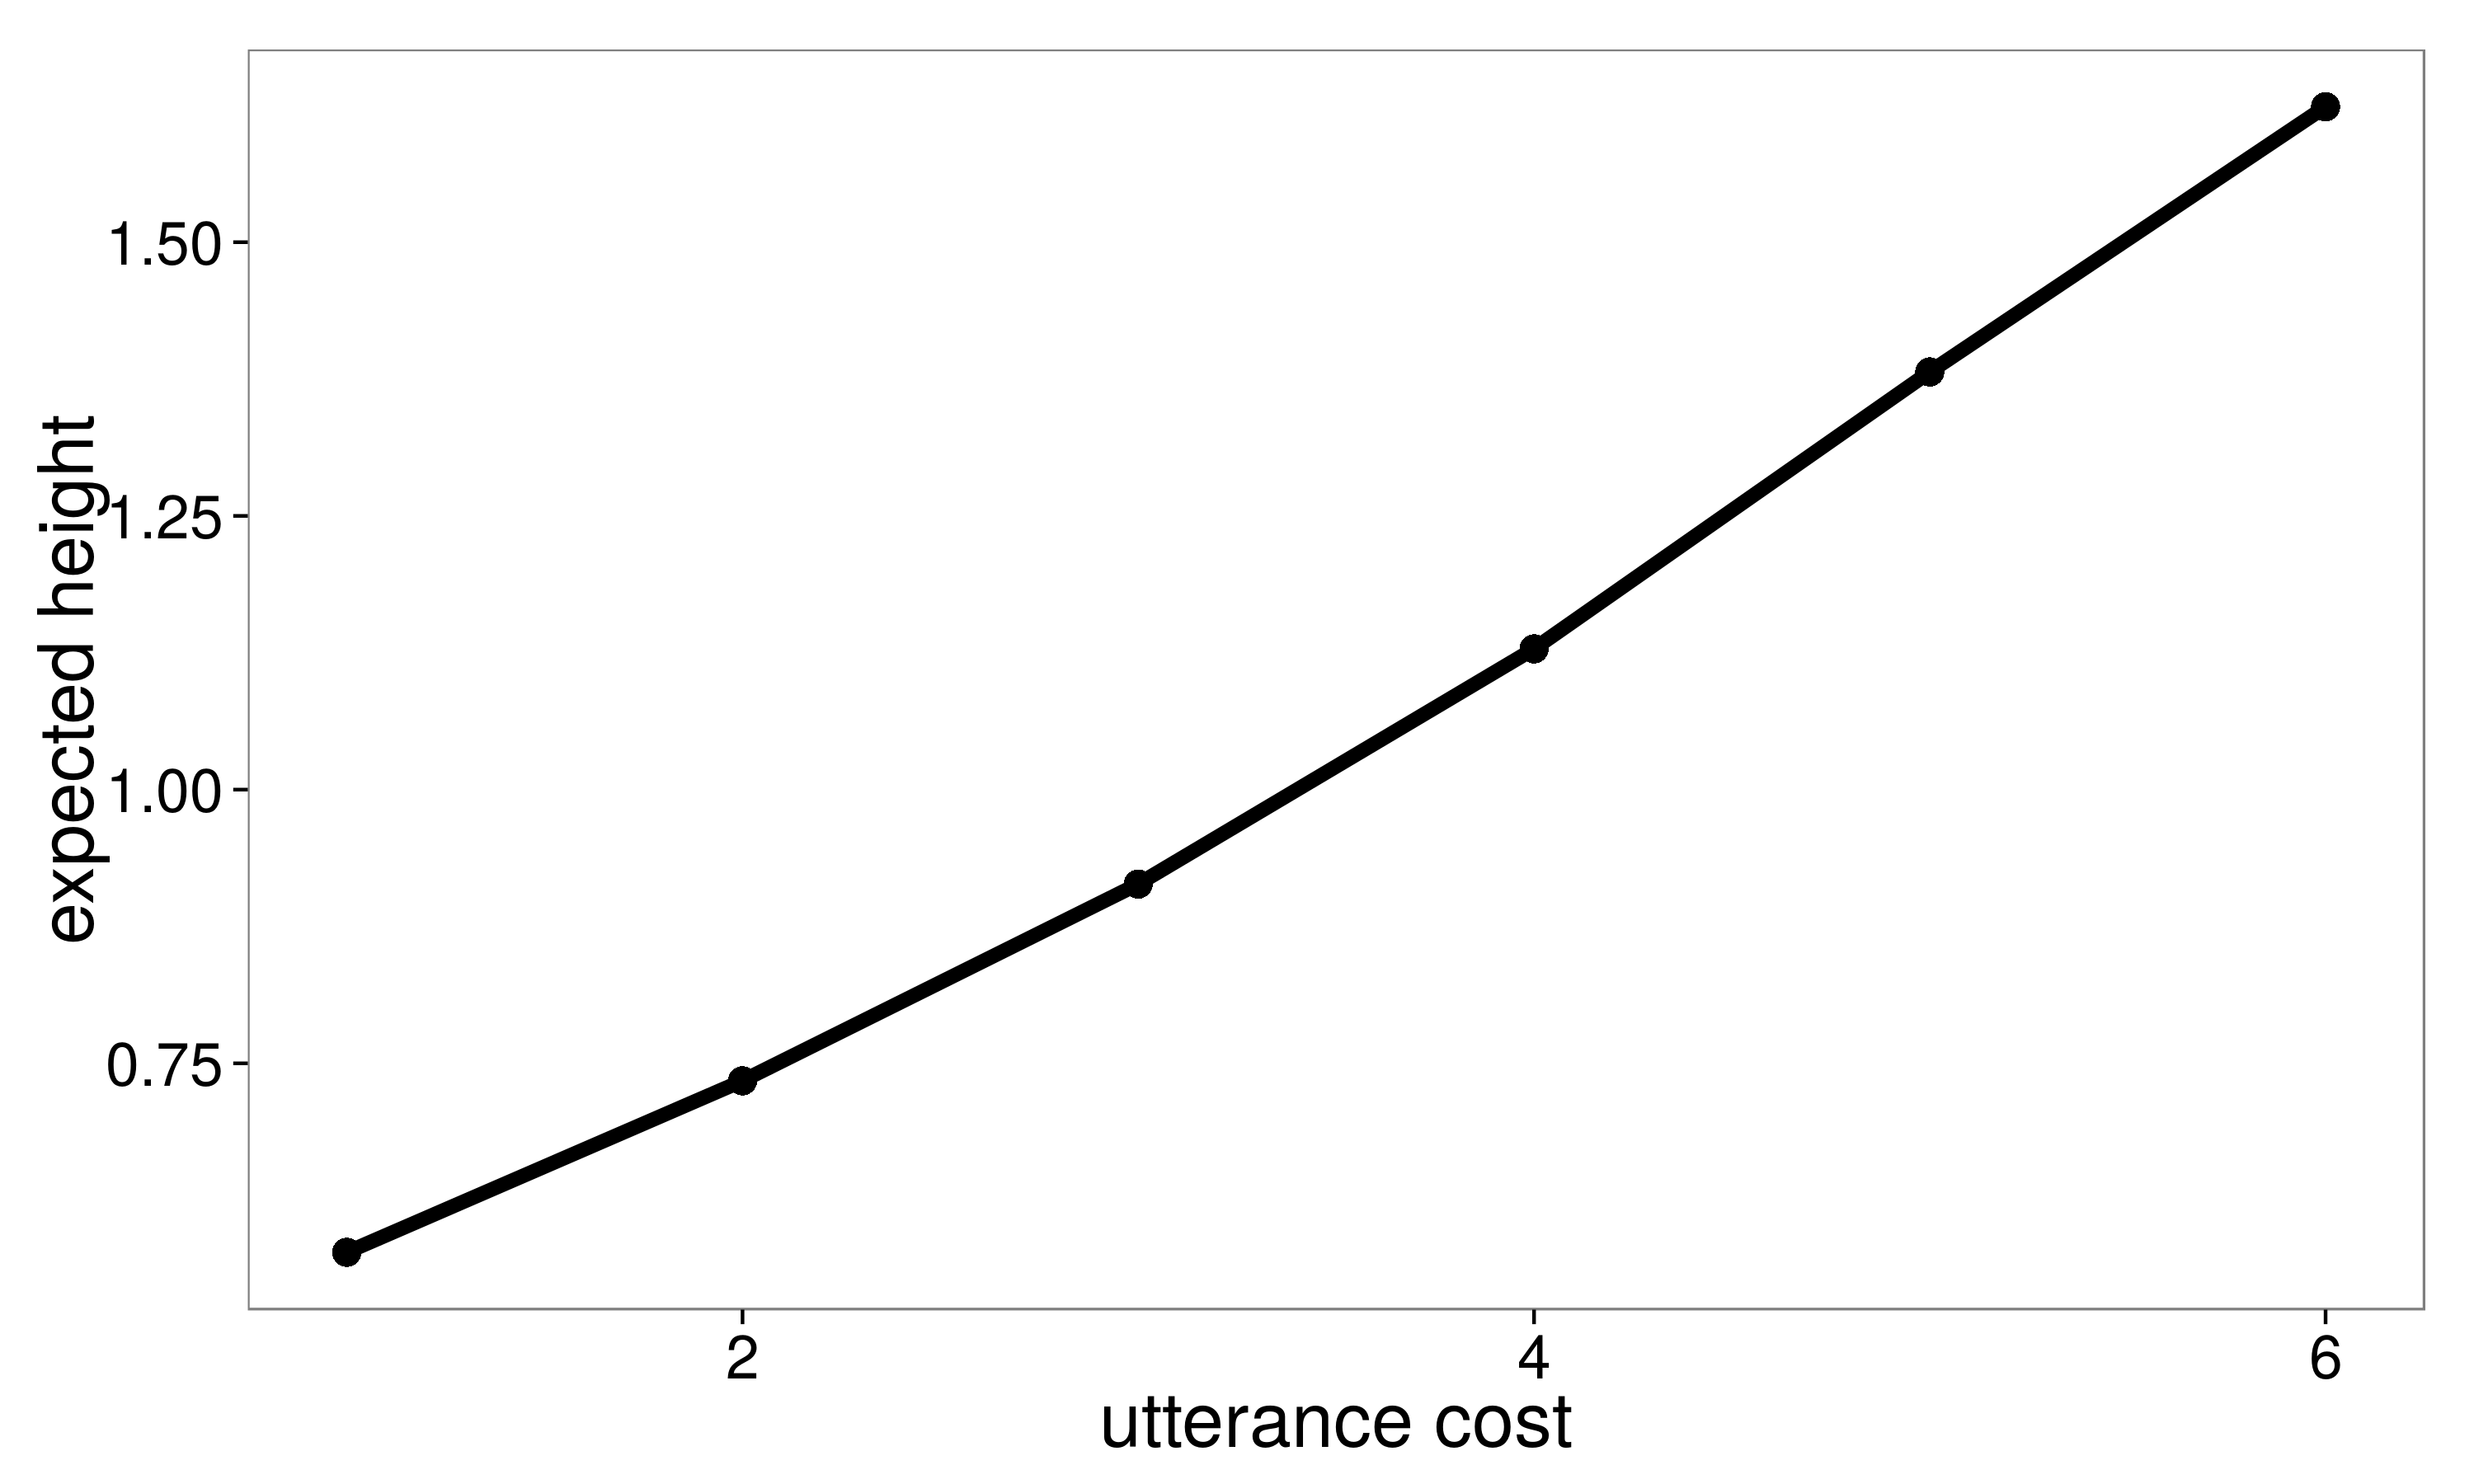
\includegraphics[width=0.4\textwidth]{analysis_files_for_writeup/images/height-by-cost.png}
\end{center}
\caption{Model prediction of expected price as cost of intensifier increases, based on intensifiers evenly spaced in cost. The relationship is approximately linear.} 
\label{model-heights}
\end{figure}

\section{Experiment 1}

The proposal detailed above predicts an association between measures of cost and strength of interpretations. In Experiment 1, we test this qualitative prediction
by eliciting free response price estimates from people and determining whether these prices are correlated with our independent measures of utterance cost.

\subsection{Method\footnote{The full experiment can be found at \url{http://cocolab.stanford.edu/cogsci2015/intensifiers/Experiment1}}}

40 participants with US IP addresses were recruited through Amazon's Mechanical Turk and paid \$0.40 for their participation.

We asked participants to estimate the prices of different objects based on different descriptions of those objects. The descriptions included intensifiers paired with the adjective \w{expensive} (Figure~\ref{exp1-q}).
There were three categories of objects (\emph{laptop}, \emph{watch}, and \emph{coffee maker}) and 40 intensifiers (see Table~\ref{exp1-intensifiers}).
We chose intensifiers that have a wide range of frequencies and excluded intensifiers that are either more commonly used to signal affect than to signal degree (e.g. ``depressingly expensive'' might indicate a degree, but it mainly indicates affect) or are ambiguous between other parts of speech (e.g. ``super'' can be used as an intensifier, as in ``super expensive'', but it can also be used as an adjective, as in ``super hero'').
Each particpant gave price judgments for every intensifier-category pairing in a randomized order (different for different participants), for a total of 120 price judgments per participant.
We chose the domain of price and used only the adjective \w{expensive} because price constitutes a quantitative scale with standard units (dollars for our US participants) on which to measure the different intensifers.

\begin{figure}[ht]
\begin{center}
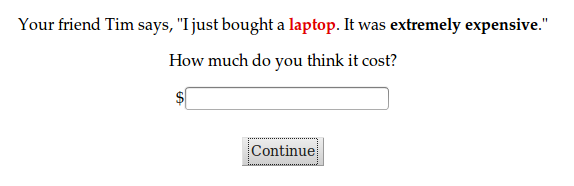
\includegraphics[width=0.4\textwidth]{analysis_files_for_writeup/images/exp1-q.png}
\end{center}
\caption{Screenshot from Experiment 1 target question.} 
\label{exp1-q}
\end{figure}

\begin{table}[ht]
 \begin{center}
 \footnotesize
  \caption{Intensifiers from Experiment 1, number of occurences in Google Web 1T 5grams corpus, and number of syllables.}
  \label{exp1-intensifiers}
  \begin{tabular}{ccc}
   \hline
   ngram & frequency & syllables \\
    \hline
    surpassingly & 11156 & 4 \\
    colossally & 11167 & 4 \\
    terrifically & 62292 & 4 \\
    frightfully & 65389 & 3 \\
    astoundingly & 73041 & 4 \\
    phenomenally & 120769 & 5 \\
    uncommonly & 135747 & 4 \\
    outrageously & 240010 & 4 \\
    fantastically & 250989 & 4 \\
    mightily & 252135 & 3 \\
    supremely & 296134 & 3 \\
    insanely & 359644 & 3 \\
    strikingly & 480417 & 3 \\
    acutely & 493931 & 3 \\
    awfully & 651519 & 3 \\
    decidedly & 817806 & 4 \\
    excessively & 877280 & 4 \\
    extraordinarily & 900456 & 6 \\
    exceedingly & 977435 & 4 \\
    intensely & 1084765 & 3 \\
    markedly & 1213704 & 3 \\
    amazingly & 1384225 & 4 \\
    radically & 1414254 & 3 \\
    unusually & 1583939 & 4 \\
    remarkably & 1902493 & 4 \\
    terribly & 1906059 & 3 \\
    exceptionally & 2054231 & 5 \\
    desperately & 2139968 & 3 \\
    utterly & 2507480 & 3 \\
    notably & 3141835 & 3 \\
    incredibly & 4416030 & 4 \\
    seriously & 12570333 & 4 \\
    truly & 19778608 & 2 \\
    significantly & 19939125 & 5 \\
    totally & 20950052 & 3 \\
    extremely & 21862963 & 3 \\
    particularly & 41066217 & 5 \\
    quite & 55269390 & 1 \\
    especially & 55397873 & 4 \\
    very & 292897993 & 2
  \end{tabular}
 \end{center}
\end{table}

\subsubsection{Corpus Methods}

Table~\ref{exp1-intensifiers} shows word frequency and length in syllables for the intensifiers used in the experiment.
The frequencies were collected from the Google Web 1T 5-grams database \cite{web1t5gram}\footnote{
We also ran the same analyses on frequency information collected from the Google Books American Ngrams Corpus \cite{books2011} and found similar results.
}
In the analysis below we use word length and word surprisal (negative log-frequency) as proxies for a word's cost, as motivated above.
The syllable lengths of our intensifiers and the surprisals %\todo[inline]{say what surprisal is and why we care before using it.} 
were correlated, but not strongly so (r = 0.27).

\subsection{Results and Discussion}

If the meaning of an intensifier is stronger for higher cost intensifiers, we would expect to find that as surprisal increases and length in syllables increases, the prices participants give will also increase. We find that this is the case.
%% what's the alternative hypothesis?

\begin{figure*}[ht]
\begin{center}
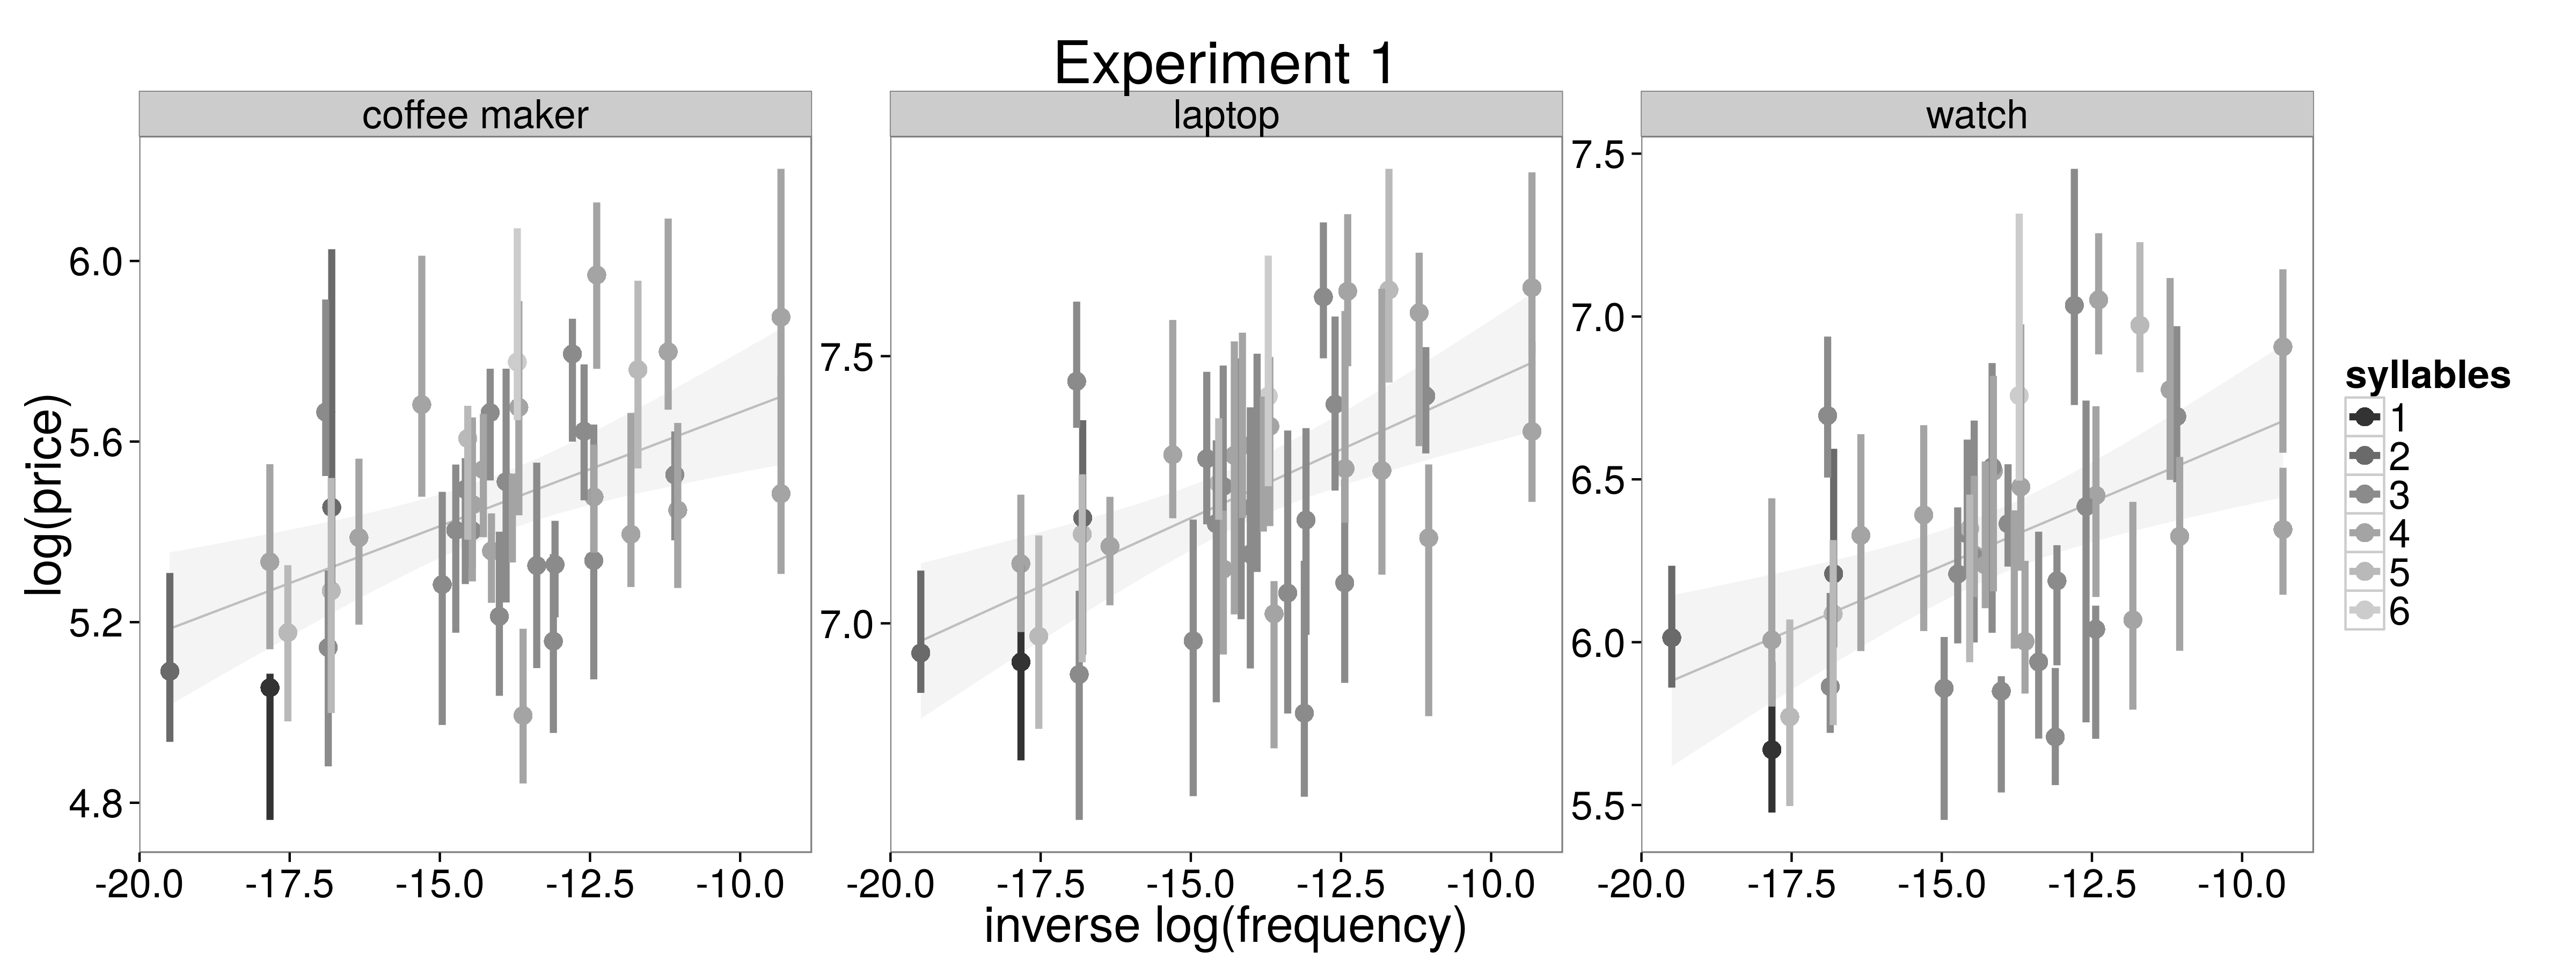
\includegraphics[width=0.8\textwidth]{analysis_files_for_writeup/images/exp1-plot.png}
\end{center}
\caption{Results of Experiment 1. As surprisal and length in syllables increase, participants' free response prices increased.} 
\label{exp1-plot}
\end{figure*}

We ran a linear mixed effects regression with centered fixed effects of syllables, surprisal, and their interaction, and random intercepts and slopes for syllables and surprisal for both participant and object.
We used the logarithm of participants' price estimates as the dependent variable, because of evidence that people's representation of numbers, including prices, is logarithmic \cite[e.g.]{dehaene}\footnote{I.e. the perceptual distance between two prices the same dollar amount apart is more for small numbers (e.g. \$3 and \$6) and less for large numbers (e.g. \$1,543 and \$1,546).}.
%of evidence that people represent differences in number logarithmically
%people's representations of numbers is logarithmic \cite{}.

%anything more complicated won't converge
% Fixed effects:
%                          Estimate Std. Error        df t value Pr(>|t|)    
% (Intercept)             6.327e+00  5.260e-01 2.000e+00  12.029 0.005051 ** 
% c.surprisal             5.365e-02  9.349e-03 3.000e+00   5.739 0.011874 *  
% c.syllables             9.311e-02  1.821e-02 5.000e+00   5.112 0.004134 ** 
% c.surprisal:c.syllables 1.931e-02  5.149e-03 3.533e+03   3.750 0.000179 ***
Our results are shown in Figure~\ref{exp1-plot}. Both measures of cost play a role in predicting participants' price estimates. We found a significant main effects of surprisal ($\beta=0.0537, SE=0.00935, t(3)=5.74, p<0.05$) such that less frequent words tend to be associated with higher price estimates. We also found a significant main effect of syllable length ($\beta=0.0931, SE=0.0182, t(5)=5.112, p<0.005$), above and beyond surprisal, such that longer words predict stronger meanings. We also found a significant interaction ($\beta=0.0193, SE=0.00515, t(3.5)=3.75, p<0.0005$) between surprisal and syllable length, wich may indicate that the relationship between the two predictors of cost is not simply additive, and that having multiple sources of communicative cost (i.e. length and surprisal) might increase the implicature even more.

Thus intensifiers that are less frequent and longer (and therefore are more costly to utter) also tend to be interpreted as having stronger meanings, at least when used to modify \emph{expensive}. Furthermore, the relationship appears to be linear in surprisal and length (though with an interaction), as predicted.
This is consistent with the M-implicature model introduced above.

\section{Experiment 2}

The M-implicature account described above implies that there is no semantic interaction between the intensifier and the adjective it is applied to. Instead an intensifier should contribute similar cost, and therefore meaning, to the different adjectival phrases in which it occurs\footnote{If the bigram frequency of the modified adjective (``very expensive'') deviated from that expected based on independent word frequencies our frequency-based cost account would predict an interactive effect on meaning. This would be a relatively small effect, and the relevant bigrams were too sparse in our corpora to pursue.}.
To explore this issue, we would like to extend our results to additional adjectival scales. However, most scales are not so easily quantifiable as price; we require a different dependent measure in order to probe them.
For Experiment 2 we used a forced-ranking dependent measure, which allows us to consider additional adjectival scales. This dependent measure has the added benefit of providing a more sensitive measure of the differences in degrees between similar adjectival phrases.

\subsection{Method\footnote{The full experiment can be found at \url{http://cocolab.stanford.edu/cogsci2015/intensifiers/Experiment2}}}

30 participants with US IP addresses were recruited through Amazon's Mechanical Turk and paid \$0.40 for  participation.

We asked participants to order (by clicking and dragging) various adjective phrases with the same adjective but different intensifiers according to strength of meaning. Because arranging these phrases required participants to be aware of the full set of adjective phrases and access all of them on the same computer screen (which might vary in size for different participants), not all of our 40 intensifiers could effectively be presented at once. We divided the 40 intensifiers from Experiment 1 into four lists of 10 intensifiers. 
%(Table~\ref{exp2-intensifiers}).
Each list was randomly paired with one of four adjectives (\w{old}, \w{expensive}, \w{beautiful}, and \w{tall}).
For each adjective-list pairing, participants were shown every combination of the 10 intensifiers with one adjective.
Participants were asked to move the adjective phrases from the left to the right side of the screen, reordering the phrases from the ``lowest'' to the ``highest'' degree (Figure~\ref{exp2-q}).
Each participant completed four such trials, seeing all four lists and all four adjectives.
The pairings between list and adjective were randomized between participants.
The division of the intensifiers into lists of 10 was constant, so that the same 10 intensifiers were always shown together to simplify data analysis.

\begin{figure}[ht]
\begin{center}
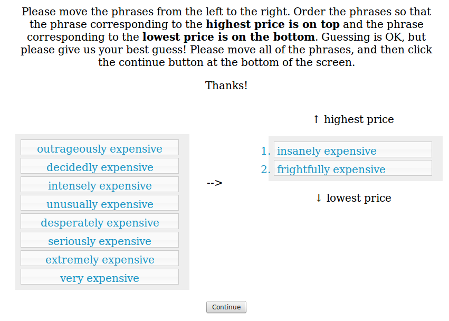
\includegraphics[width=0.4\textwidth]{analysis_files_for_writeup/images/exp2-q.png}
\end{center}
\caption{Screenshot from Experiment 2 target question.} 
\label{exp2-q}
\end{figure}

%\begin{table}[ht]
%\begin{center} 
%\footnotesize
%\caption{Intensifier Lists from Experiment 2: Rankings.} 
%\label{exp2-intensifiers} 
%\vskip 0.12in
%%\scalebox{0.3}{
%\begin{tabular}{cccc} 
%\hline
%List A    &  List B & List C & List D \\
%\hline
%surpassingly & colossally & terrifically & frightfully \\
%astoundingly & phenomenally & uncommonly & outrageously \\
%fantastically & mightily & supremely & insanely \\
%strikingly & acutely & awfully & decidedly \\
%excessively & extraordinarily & exceedingly & intensely \\
%markedly & amazingly & radically & unusually \\
%remarkably & terribly & exceptionally & desperately \\
%utterly & notably & incredibly & seriously \\
%truly & significantly & totally & extremely \\
%particularly & quite & especially & very
%\end{tabular}
%%}
%\end{center}
%\end{table}

\subsection{Results and Discussion}
%                          Estimate Std. Error  z value  Pr(>|z|)    
% c.surprisal              0.318717   0.024710  12.8982 < 2.2e-16 ***
% c.syllables              0.437042   0.065800   6.6420 3.095e-11 ***
% c.surprisal:c.syllables  0.040977   0.023601   1.7362   0.08253 . 
Our results for Experiment 2 are shown in Figure~\ref{exp2-plot}. We ran an ordinal
regression with centered surprisal and syllable lengths and their interaction as fixed effects.
As in Experiment 1, we found strong main effects of surprisal ($\beta=0.319, SE=0.0247, t=12.9, p<5e-38$) and syllable length ($\beta=0.437, SE=0.0658, t=6.64, p<5e-11$), with only a trending interaction ($p=0.0825$).
In other words, we again found that participants assign stronger interpretations to intensifiers with higher surprisals and/or higher syllable lengths, extending now across four different adjectival scales.
%could say something more about these results? interaction between intensifier and adjective?

\begin{figure*}[ht]
\begin{center}

\includegraphics[width=0.8\textwidth]{analysis_files_for_writeup/images/exp2-plot.png}
\end{center}
\caption{Results of Experiment 2. As surprisal and length in syllables increase, participants' rankings increased.} 
\label{exp2-plot}
\end{figure*}

\section{General Discussion}

Motivated by a recent probabilistic model of scalar adjectives \cite{lassiter}, we showed how adjectival intensifiers could potentially get their meaning through a pragmatic M-implicature, despite having vacuous literal meaning to add to an adjective. Our model predicted a linear relationship between the intensity of an intensifier and its cost, measured here in terms of length and log-frequency.
In two experiments we provided evidence that intensifier meanings do depend systematically on the length and frequency of distribution of those word forms.
While it is unlikely that this accounts for all intensifier meaning, it does suggest that a major portion of meaning comes not from arbitrary, conventional association of signal to sign \cite{saussure}, but from features of the word's form and distribution.

It should be noted that, since this is a correlational study, such a relationship does not confirm that an intensifier's cost \emph{causes} it to have a given meaning. This correlation is predicted by the model sketched above, but it might be predicted by other analyses of intensifiers and their meanings. Rarity in particular might be correlated with strength of meaning merely because more extreme meanings refer to less probable things in the world, are therefore talked about less, and therefore the words with those meanings will necessarily be rarer.
%% this next bit is sketch
Although it seems reasonable to suspect that word frequencies reflect the probabilities of the real-world concepts they describe, it might also be the case that improbable things are more likely to be commented on, and so to a certain extent the frequencies of words that describe rare concepts will be inflated. Even so, this confound exists only for word frequency and not for syllable length.
%citation?
The length of a word seems much less likely to reflect the real-word prevalence of the concept it refers to.

A number of issues remain to future work, including the causality of the relationship we have described and the other aspects of intensifier meaning (such as polarity or affective color).
However we believe that the preliminary results presented in this paper already have interesting implications. 
For the semantics of adverbial modifiers, we have shown how pragmatic mechanisms could be central in establishing flexible contributions to sentence meaning.
For the broader question of form-meaning mapping, we have suggested a source of non-arbitrary association based on both properties of the word form and of its distribution.

%%%%awesome, but too detailed for here:
%We could also investigate other sources of commicative cost. \citeA{peters} %Peters (1994)
%notes that, since intensifiers often originate as qualitative adverbs and gradually shift to being primarily adverbs of degree (e.g. terribly once only carried the qualitative meaning of ``bad and frightening'', but now almost exclusively means simply ``a lot''), interlocuters might have to resolve ambiguity about which sense of the adverb is intended and that resolving this ambiguity could be cognitively demanding. So intensifiers that are newer and less conventially used to signal degree, like \w{skyscrapingly}, would incur higher communicative cost to the comprehender (in disambiguating) and to the speaker (in choosing a less common meaning, or creatively generating a new intensifier) than something more commonly used to signal degree, like \w{very}.\footnote{The extent to which an adverb is used as an intensifier as opposed to as a qualitative adverb can be approximated by the number of types of adjectives an adverb can coocur with. The more freely it is able to pair with arbitrary adverbs, the more likely its conventional meaning is one of degree as opposed to quality.}
%%%maybe move that to the discussion
%make it sound like ``this is a reasonable thing to do.
%then in the discussion say, ''that was reasonable, but there are other reasonable things. for example:
%%%maybe this should be a footnote:
%%%%%%The extent to which a degree adverb (e.g. \w{terribly}) takes a degree interpretation (e.g. ''a lot`` as opposed to ''this sucks``) can be approximated by the extent to which it 
%the number of different types of adjetives that it coocurs with
%freely collocates with a variety of adjectives, since adverbs that are more qualitative will have more restricted collocations.

%\todo[inline]{if room could say something about next steps. also relation to other's work on meaning.}

%``my paper is totally done'' when you expect it to be done: might actually mean that it's almost done.

%\section{Acknowledgments} %%NDG: add in camera ready

\bibliographystyle{apacite}

\setlength{\bibleftmargin}{.125in}
\setlength{\bibindent}{-\bibleftmargin}

\bibliography{intensifiers}

\end{document}
